\id{МРНТИ 28.23.29}{}

\begin{articleheader}
\sectionwithauthors{А. Даулеткалиева, А. Муканова, А. Назырова, Б. Ергеш, Л. Жеткенбай, А. Бурибаева}{ИЗВЛЕЧЕНИЕ СЕМАНТИЧЕСКИХ ДАННЫХ ИЗ ТЕКСТОВ НА ОСНОВЕ БОЛЬШИХ ЯЗЫКОВЫХ МОДЕЛЕЙ}

{\bfseries
\textsuperscript{1}А. Даулеткалиева\alink{https://orcid.org/0009-0001-6106-8776}\textsuperscript{\envelope },
\textsuperscript{1}А. Муканова\alink{https://orcid.org/0000-0002-8964-3891},
\textsuperscript{2}А. Назырова\alink{https://orcid.org/0000-0002-9162-6791},
\textsuperscript{2}Б. Ергеш\alink{https://orcid.org/0000-0002-8967-2625},
\textsuperscript{2}Л. Жеткенбай\alink{https://orcid.org/0000-0001-9843-6125},
\textsuperscript{1}А. Бурибаева\alink{https://orcid.org/0009-0008-6374-6447}
}
\end{articleheader}

\begin{affiliation}
\textsuperscript{1}Международный университет Астана, Астана, Казахстан,

\textsuperscript{2}«Евразийский национальный университет им. Л.Н. Гумилева», Астана, Казахстан

\raggedright \textsuperscript{\envelope }Корреспондент-автор: assem.dauletkaliyeva1@gmail.com
\end{affiliation}

В процессе применения технологии есть несколько взаимосвязанных этапов.
Сначала из текста выбирается информация, имеющая смысловое значение.
Затем они приводятся в определенную структуру и включаются в
онтологическую модель. На последнем этапе между этими данными
устанавливаются семантические связи в результате формирования внутренней
структуры онтологической системы.

Кроме того, метод был протестирован на онтологической модели,
описывающей административно-географические особенности Казахстана. Опыт
показал, что этот подход может быть эффективно применен не только в
конкретной области, но и в других областях, таких как здравоохранение,
многомерный анализ текстовых данных.

Результаты исследования показали, что предложенный подход позволяет
систематизировать сложные текстовые структуры и вносить их в базу
знаний. В этой области этот метод может играть особенно важную роль в
разработке интеллектуальных систем, особенно в проектах, предназначенных
для автоматической обработки и интерпретации сложных знаний.

{\bfseries Ключевые слова:} онтологическая модель, извлечение данных, LLM,
ChatGPT, семантическая сеть, OpenAI API.

\begin{articleheader}
{\bfseries EXTRACTING SEMANTIC DATA FROM TEXTS BASED ON LARGE LANGUAGE MODELS}

{\bfseries
\textsuperscript{1}A. Dauletkaliyeva\textsuperscript{\envelope },
\textsuperscript{1}A. Mukanova,
\textsuperscript{1}A. Nazyrova,
\textsuperscript{2}B. Yergesh,
\textsuperscript{2}L. Zhetkenbai,
\textsuperscript{1}A. Buribayeva
}
\end{articleheader}

\begin{affiliation}
\textsuperscript{1}Astana International University, Astana, Kazakhstan,

\textsuperscript{2}L.N. Gumilyov Eurasian National University, Astana, Kazakhstan,

е-mail: assem.dauletkaliyeva1@gmail.com
\end{affiliation}

There are several interrelated stages in the process of applying the
technology. First, information with semantic meaning is selected from
the text. Then they are brought into a certain structure and included in
the ontological model. At the last stage, semantic connections are
established between these data as a result of the formation of the
internal structure of the ontological system.

In addition, the method was tested on an ontological model describing
the administrative and geographical features of Kazakhstan. Experience
has shown that this approach can be effectively applied not only in a
specific field, but also in other areas such as healthcare,
multidimensional text data analysis.

The results of the study showed that the proposed approach makes it
possible to systematize complex text structures and add them to the
knowledge base. In this field, this method can play a particularly
important role in the development of intelligent systems, especially in
projects designed for the automatic processing and interpretation of
complex knowledge.

{\bfseries Keywords:} оntological model, data extraction, LLM, ChatGPT,
semantic network, OpenAI API.

\begin{articleheader}
{\bfseries ҮЛКЕН ТІЛДІК МОДЕЛЬДЕР НЕГІЗІНДЕ МӘТІНДЕРДЕН СЕМАНТИКАЛЫҚ ДЕРЕКТЕРДІ АЛУ}

{\bfseries
\textsuperscript{1}А. Даулеткалиева\textsuperscript{\envelope },
\textsuperscript{1}А. Муканова,
\textsuperscript{2}А. Назырова,
\textsuperscript{2}Б. Ергеш,
\textsuperscript{2}Л. Жеткенбай,
\textsuperscript{1}А. Бурибаева
}
\end{articleheader}

\begin{affiliation}
\textsuperscript{1}Астана халықаралық университеті, Астана, Қазақстан,

\textsuperscript{2}Л.Н.Гумилев атындағы Еуразия ұлттық университеті, Астана, Қазақстан,

е-mail: assem.dauletkaliyeva1@gmail.com
\end{affiliation}

Технологияны қолдану процесінде бірнеше өзара байланысты кезеңдер бар.
Алдымен мәтіннен семантикалық мағынасы бар ақпарат таңдалады. Содан
кейін олар белгілі бір құрылымға келтіріліп, онтологиялық модельге
енгізіледі. Соңғы кезеңде онтологиялық жүйенің ішкі құрылымын
қалыптастыру нәтижесінде осы мәліметтер арасында семантикалық
байланыстар орнатылады.

Сонымен қатар, әдіс Қазақстанның әкімшілік-географиялық ерекшеліктерін
сипаттайтын онтологиялық модельде сыналды. Тәжірибе көрсеткендей, бұл
тәсілді тек белгілі бір салада ғана емес, денсаулық сақтау, мәтіндік
деректерді көп өлшемді талдау сияқты басқа салаларда да тиімді қолдануға
болады.

Зерттеу нәтижелері ұсынылған тәсіл күрделі мәтіндік құрылымдарды
жүйелеуге және оларды білім базасына енгізуге мүмкіндік беретіндігін
көрсетті. Бұл салада бұл әдіс интеллектуалды жүйелерді дамытуда, әсіресе
күрделі білімді автоматты түрде өңдеуге және түсіндіруге арналған
жобаларда ерекше маңызды рөл атқаруы мүмкін.

{\bfseries Түйін сөздер:} онтологиялық модель, деректерді алу, LLM,
ChatGPT, семантикалық желі, OpenAI API.

\begin{multicols}{2}
{\bfseries Введение.} Поток информации, который ежедневно окружает нас,
давно вышел за рамки простого «много данных». Изображения, видео, тексты
и звук - всё это не просто хранится в цифровом пространстве, а
обновляется каждую секунду. Но удивительно другое: несмотря на то, что
данные есть, их понять - особенно машине - всё ещё сложно. Почему? Да
потому что большинство из них неструктурированы. Они не объясняют себя,
не говорят, что в них важно и главное - не несут ясного смысла,
доступного для алгоритмов.

Да, у нас есть распознавание лиц, машинный перевод, поиск по картинкам.
Но всё это похоже на то, как если бы вы узнали слово, но не поняли, что
оно значит в разговоре. Контекст ускользает. А значит -ускользает и
понимание.

Вот почему всё чаще говорят об онтологиях. Это не просто модное слово -
это способ навести порядок. Представьте карту, где каждое понятие
связано нитями с другими, где всё не хаотично, а продумано {[}1, 2{]}.
Именно так компьютер начинает не просто читать данные, а, если угодно,
понимать, о чём речь.

Онтологические модели ценятся за их гибкость-их можно уточнять,
перестраивать, комбинировать с другими. Это не только сохраняет
информацию, но и создает целые системы знаний, которые развиваются и
обогащаются с течением времени {[}3{]}.

Над онтологией часто работают несколько команд: десятки специалистов из
разных организаций объединяют усилия. Специальные пространства имен
используются для того, чтобы их фрагменты не мешали друг другу и в то же
время взаимодействовали. Такой подход помогает сохранить независимость
каждой части и в то же время связать их друг с другом {[}4{]}.

Семантическая сеть предлагает переосмысление сущности Интернета. Он не
только связывает документы, но и превращает различную информацию в
единую сеть значений. В такой системе поиск становится интеллектуальным,
а данные взаимосвязаны. Это уже не просто чтение, а понимание.

На практике онтологии доказали свою ценность на гораздо более высоком
уровне, чем наука. Они используются при создании экспертных платформ,
публикации связанных данных, образовательных систем и образовательных
проектов {[}5{]}.

Но в этой разработке есть одно "но" - большая часть информации еще не
заказана. Пока мы не знаем, как автоматически преобразовывать
хаотические данные в структурированные данные, еще слишком рано говорить
о полном "понимании" со стороны машин.

Здесь запускаются системы получения информации. Их задача-найти главное
в тексте, отбросить лишнее и построить логическую структуру. Только
тогда данные будут действительно полезны для интеллектуальной обработки.

Интернет пестрит данными, но вот найти среди них действительно ценную
информацию - задача, которую не всегда под силу даже человеку, не говоря
уже о машине. HTML-страницы могут быть переполнены деталями, но далеко
не всё, что там есть, представляет интерес. Алгоритмам приходится
отделять шум от сути, и именно здесь начинаются сложности.

Контекст ускользает. Слова теряют смысл без окружения. Машинам не
хватает «чутья», чтобы понять, к чему относится то или иное утверждение.
А если в тексте встречаются намёки, ирония или двусмысленность - считай,
алгоритм попал в тупик.

В условиях, когда информация собирается в невероятных объёмах, но
остаётся хаотичной, становится ясно: без надёжных методов обработки ни о
каком осмысленном использовании речи быть не может. В этой статье речь
пойдёт о том, как современные подходы помогают сделать знания доступными
для машин - и какие идеи могут изменить ландшафт цифровой обработки в
ближайшие годы.

{\bfseries Обзор литературы}. Большие языковые модели в последние годы
стали настоящим прорывом в области онтологического обогащения. Если
раньше извлечение знаний из текстов требовало кропотливой работы
экспертов, то теперь эту задачу можно частично передать алгоритмам. Они
всё лучше справляются с тем, чтобы находить в неструктурированных
текстах действительно полезную информацию и превращать её в элементы
формализованных моделей.

Одним из направлений, вызвавших большой интерес, стало межъязыковое
сопоставление. Например, в методике, предложенной Ибрагимом и его
коллегами, используется семантическое выравнивание для автоматического
расширения онтологий. Алгоритм сам подбирает наиболее уместные переводы
терминов - подход, который особенно важен в условиях многоязычной среды
{[}6{]}.

Методы глубинного обучения тоже не остались в стороне. В частности,
работа Санагаварапу и его команды показывает, как алгоритмы анализируют
текстовые данные из открытых баз по уязвимостям и профильных форумов.
Это особенно актуально для сфер вроде кибербезопасности, где важно
быстро находить и обновлять знания в онтологиях {[}7{]}.

Вероятностные подходы дают интересный результат, особенно при работе с
разнородными источниками. Так, в системе, описанной Тиссауи с
соавторами, используется тематическое моделирование - оно позволяет
выявлять скрытые связи и строить терминологические онтологии без жёсткой
ручной настройки {[}8{]}.

Как отмечают Кокла и его коллеги, онтологии дают возможность существенно
повысить точность семантического поиска. Благодаря аннотированию и
структурированному представлению информации пользователи быстрее находят
релевантные данные {[}9{]}.

Особую роль сейчас начинают играть решения, которые позволяют не просто
обновлять знания, а связывать их между собой. Например, система,
созданная Себуби, строится на принципах связных данных и помогает
автоматически интегрировать новые фрагменты знаний, при этом сохраняя
целостность онтологической структуры {[}10{]}.

Область автоматического сопоставления онтологий продолжает развиваться.
Особенно интересной стала возможность подключить большие языковые
модели. Без предварительной разметки, всего по паре примеров, такие
модели уже показывают неплохие результаты. Хертлинг, к примеру,
продемонстрировал, что zero-shot и few-shot методы вполне способны
заменить традиционные алгоритмы, требующие большого количества обучающих
данных {[}11{]}.

Это не просто удобство - это смена подхода. Мы переходим к новым
принципам управления знаниями. Здесь вместе работают вероятностные
методы, машинное обучение и межъязыковая семантика. Всё это помогает
строить онтологии, которые могут меняться и расти по мере поступления
новых данных.

Тем не менее, далеко не всё исследовано. Например, тема использования
LLM и отечественных ИИ-систем в таких узких областях, как
геоинформационные технологии, почти не затронута. Здесь пока пробел, и
он явно требует внимания - как со стороны исследователей, так и
разработчиков.

{\bfseries Материалы и методы.} Одного инструмента может быть недостаточно.
Чтобы выжать максимум из текста, пришлось сочетать несколько технологий.
Главное - связать онтологии с обработкой естественного языка. Это дало
нужный эффект: получилось не просто анализировать фразы, а понимать, о
чём они - в машинных терминах.

Основой служила большая языковая модель (LLM). Она брала
неструктурированные тексты, переводила их в понятную системе форму, а
дальше - дело за Protégé и OWLready2: они помогали встроить извлечённую
информацию в онтологическую структуру.

Список методов оказался достаточно разнообразным: от NER и
семантического анализа до машинного обучения и логического вывода. Всё
это в комплексе помогло выстроить между понятиями такие связи, которые
руками выискивать долго и сложно. Качество проверяли не на глаз:
использовали точность, полноту и F1-оценку. Так получилась объективная
картина, а не просто впечатление. Интересно, что методика сработала не
только в одной узкой теме - её получилось адаптировать под разные
области. Это ещё раз показало: автоматический семантический анализ
способен вытянуть порядок даже из самого разрозненного текста.

{\bfseries Архитектура информационной системы для проведения эксперимента.}
Во время эксперимента без своей системы обойтись не получилось. Одних
только данных было мало - нужно было понять, как связаны между собой
понятия и как лучше с ними работать (см. рисунок 1). Для начала
построили онтологию. Использовали Protégé: задавали классы, указывали
свойства, соединяли элементы между собой. Постепенно возникла картина,
где всё логично связано. Чтобы не запутаться в связях, добавили
небольшие пояснения и ограничения. Это помогло избежать недопонимания и
позволило системе работать с моделью без ошибок.

Здесь приведён кусочек итоговой схемы. Он даёт общее представление о
том, как выстроены понятия и какие отношения между ними заложены.

\begin{figure}[H]
	\centering
	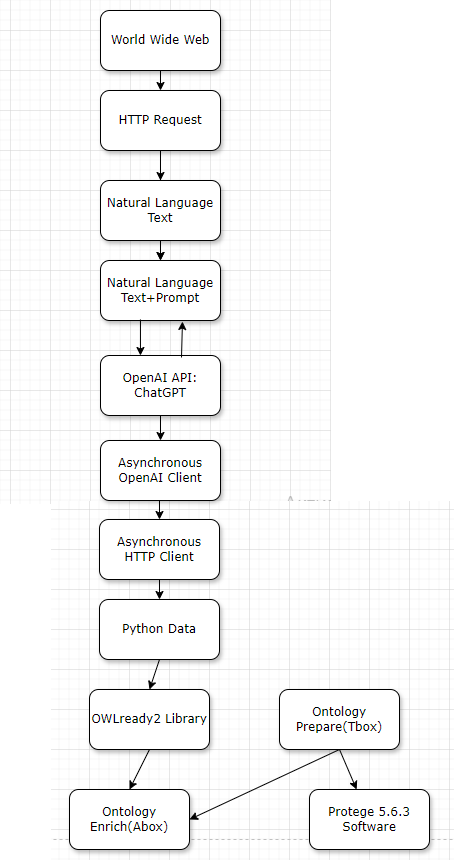
\includegraphics[width=0.4\textwidth]{media/ict2/image149}
	\caption*{Рис.1 - Архитектура информационной системы извлечения данных}
\end{figure}

Система включает приложение Python, написанное в версии 3.9. Он не
только загружает текст, его задача-извлекать смысл из материалов и
превращать его в онтологические объекты без вмешательства человека.

На начальном этапе программа получает доступ к определенному набору
ссылок. Эти адреса выбираются по теме разработанной онтологии.
Запрошенные веб-страницы содержат тексты, которые могут включать важные
термины и концепции. Таким образом, система может получить доступ к
исходному, еще не структурированному контенту.

Дается дополнительное объяснение: на каждую страницу отправляется
отдельный запрос. Он предназначен для учета специфики текстовой
презентации и формата промежуточных данных. Благодаря этому система
способна "понять", где находится главное и где находится второй уровень,
и не потерять основную информацию.

После этого собранный текст отправляется в OpenAI GPT-3.5. Из него
извлекаются структурированные фрагменты, которые возвращаются в формате
Python, часто в списках или словарях. Они служат основой для создания
онтологических объектов.

Эти объекты формируются прямо внутри системы. Через библиотеку OWLready2
им присваиваются свойства, отношения и дополнительные характеристики.
Таким образом расширяется структура онтологии: появляются новые понятия
и связи --- и все это происходит без ручной обработки.

В следующем разделе показано, как эти функции интегрированы в общую
архитектуру всей системы и как связаны отдельные модули.

{\bfseries Описание эксперимента.} Попробуйте использовать несколько
HTTP-протоколов в Интернете. Первоначальный список ссылок веб-страниц
был выявлен при участии специалиста с салат-баром.

Исходя из задач, такой подход позволял проводить семантическое
кодирование: поисковики по контенту искали любую информацию, а инженерия
онтологий на их основе формировала модель знаний.

Для извлечения данных использовалась библиотека aiohttp, которая
обеспечивает асинхронную передачу HTTP-запросов. Не забудьте установить
систему параллельно и обработать автоматом. Наряду с Sony есть и
некоторые элементы, не связанные с рекурсивной структурой веб-браузера:
баннеры, сервисные знаки, технические записи. Все эти данные были
распределены до начала работы с онтологией.

Для структурирования контента использовалась библиотека BeautifulSoup.
Он был закодирован, а основные текстовые фрагменты были объединены в
HTML-документы для создания других полезных изображений. Например, был
рассмотрен сайт Википедии «География Казахстана»
(\href{https://kk.wikipedia.org/wiki/Geography_of_Kazakhstan}{https://kk.wikipedia.org}, дата обращения
20 апреля 2024 г.). Из этой статьи были отобраны основные части текста и
создана система геоинформационной онтологии.

HTML Свяжитесь с нами (см. Гарантия 2). Алгоритм классифицирует основные
блоки и темы. Они основаны на структуре сайта, которая может быть
адаптирована к сайту. Этот метод позволил сократить количество столбцов
в онтологии, собрав в одном месте контент различных форматов.

Как читать статью в Википедии (рис.2) модель генерации chatgpt 3.5
генерирует вызов ввода, который также может включать структурированные
данные на основе инструкций на естественном языке. Основная цель
модели-автоматически извлекать и конвертировать полезный машиночитаемый
контент с соответствующих веб-сайтов в формат, соответствующий целевой
теме. Даже при использовании одного и того же входного запроса
вероятностный характер chatgpt может привести к тому, что выходные
результаты будут отличаться от запуска к запуску. Это отклонение требует
быстрой и точной структурной корректировки для обеспечения стабильности
и целостности выходных данных. Три основных компонента запроса-это код
веб-страницы, который изначально содержит неструктурированные данные,
общее описание полученных данных с указанием критериев соответствия и
описание выходного формата, которое гарантирует совместимость с
используемыми методами обработки данных.
\end{multicols}

\begin{figure}[H]
	\centering
	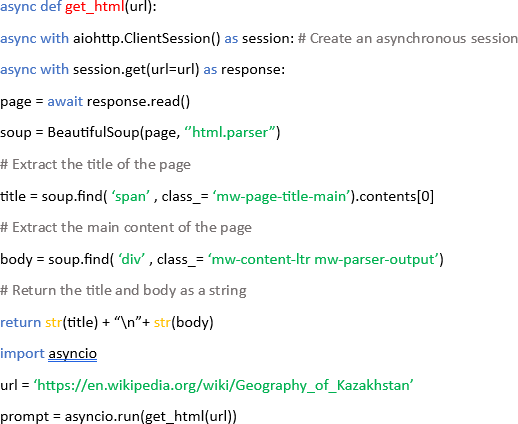
\includegraphics[width=0.5\textwidth]{media/ict2/image150}
	\caption*{Рис.2 - Анализ страницы wikipedia.org}
\end{figure}

\begin{multicols}{2}
Структуры данных Python-это предсказуемый формат представления данных.
Это значительно упрощает интеграцию информации в информационную систему.
С помощью этого метода неструктурированные тексты могут быть
автоматически преобразованы в семантически значимые структуры, которые
можно редактировать дальше. С помощью ряда тестов был разработан
идеальный формат вызова. Благодаря ему результаты хорошо повторяются. На
рисунке 3 приведен пример такой структуры вызова; код веб-страницы не
включен из-за его размера. Благодаря улучшенной структуре приглашений
результаты мало меняются. Это улучшает структуру и качество полученных
данных, что имеет решающее значение для автоматического обогащения
онтологий на основе веб-материалов.
\end{multicols}

\begin{figure}[H]
	\centering
	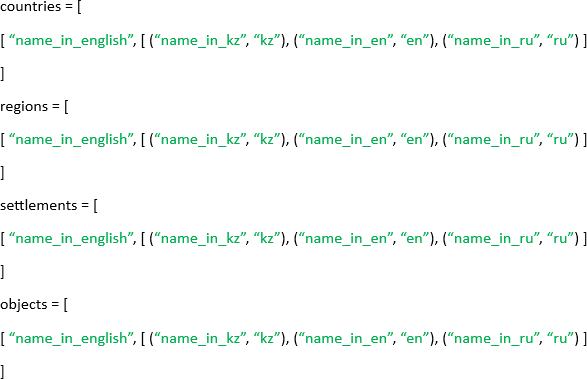
\includegraphics[width=0.5\textwidth]{media/ict2/image151}
	\caption*{Рис.3 - Запрос ChatGPT для извлечения данных с веб-страницы в списки на Python}
\end{figure}

\begin{multicols}{2}
Текстовое описание предполагаемого результата и структурный формат
представления данных, удовлетворяющий требованиям онтологической модели,
приведены в приглашении chatgpt 3.5 для обеспечения точного получения и
структурирования информации.

Целевой формат, Python, упрощает ввод полученных результатов в созданную
информационную систему.

Приглашение включает восемь списков, каждый из которых играет
определенную семантическую роль:

Люди, принадлежащие к важным классам онтологии Country, area, settlement
и object, находятся в первых пяти списках. Географическая онтологическая
модель строится с использованием этих элементов данных в качестве
основы.

Иерархические отношения между объектами определяются тремя другими
списками:

- Связь между регионами и конкретными странами устанавливается функцией
регион - страна.

- Регион-населенный пункт (определяет территориальную принадлежность
населенного пункта);

- Объект-регион: связывает объекты с соответствующими регионами, включая
памятники архитектуры или природы.

Эту систематическую методологию можно использовать для автоматизации
процесса построения онтологических моделей. Это обеспечивает машинное
чтение и последовательность полученной онтологии.

Кодифицированное описание извлеченных данных снижает вариативность
ответов генерируемой модели. Точность интерпретации информации также
улучшилась.

Пока данные извлекаются и организуются автоматически, доступ к OpenAI
API осуществляется через асинхронную библиотеку AsyncOpenAI.

Этот метод позволяет эффективно обрабатывать запросы асинхронно. Это
снижает задержку при обмене данными, особенно при обработке многих
последовательных запросов. На рисунке 4 показан компьютерный код,
показывающий, как отправить запрос с использованием экземпляра класса
OpenAIClient.
\end{multicols}

\begin{figure}[H]
	\centering
	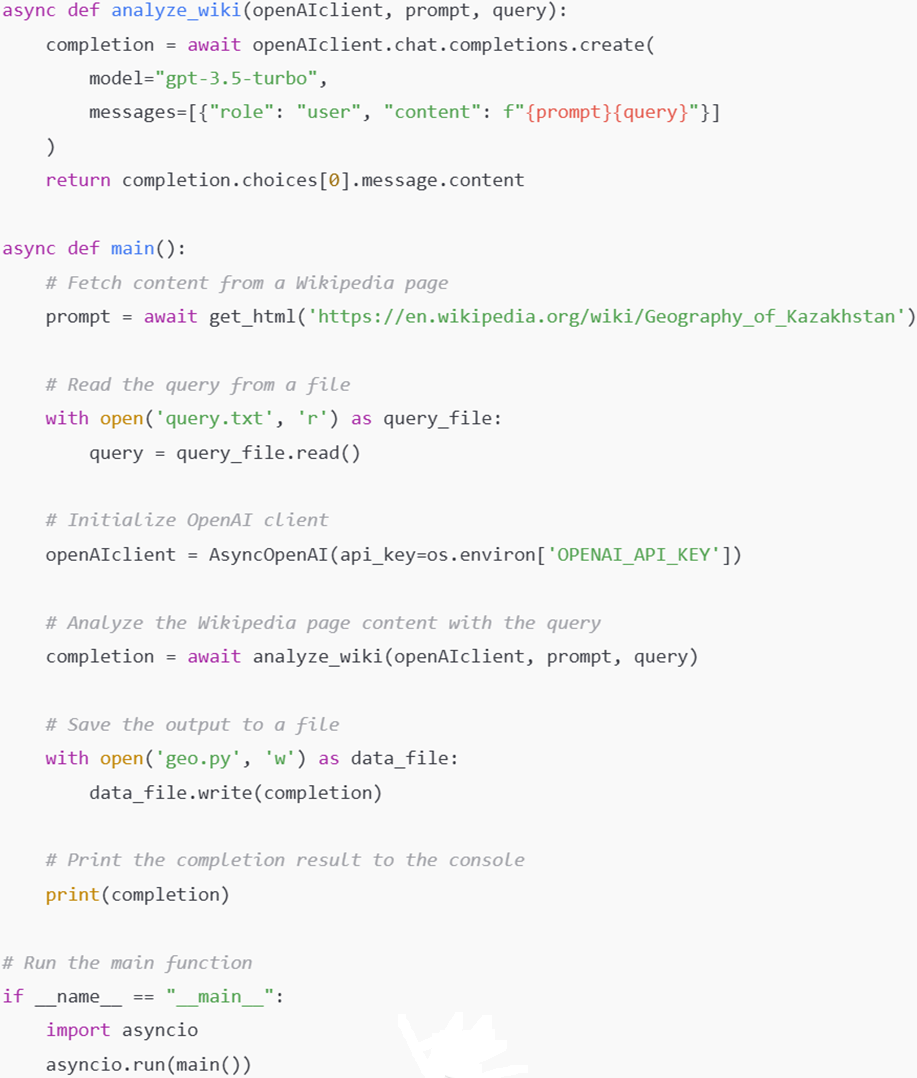
\includegraphics[width=0.6\textwidth]{media/ict2/image152}
	\caption*{Рис.4 - Отправка запроса к открытому API}
\end{figure}

\begin{multicols}{2}
Готовое приглашение ввода можно найти в текстовом файле. запрос.текст.
Запрос загружается из файла перед отправкой. Этот метод сохранения
упрощает адаптацию содержимого приглашения к конкретным требованиям
области заголовка.

Асинхронный метод взаимодействия API позволяет обрабатывать несколько
запросов одновременно. Это особенно полезно при использовании модели в
системах с высокой нагрузкой.

ChatGPT 3.5 завершает запрос и возвращает машиночитаемый ответ
(например, структуры данных JSON или Python). Это упрощает дальнейшую
обработку результатов и интеграцию в онтологическую модель.

На рисунке 5 показан код Python, созданный в результате запроса
ChatGPT-3.5. Это обеспечивает непрерывную интеграцию в рабочий процесс
обработки программного обеспечения без необходимости дальнейшего анализа
или преобразования.

Использование этой стратегии упрощает управление данными. Это позволяет
автоматически получать структурированные данные и немедленно
использовать их для дальнейшего анализа или онтологического
моделирования.
\end{multicols}

\begin{figure}[H]
	\centering
	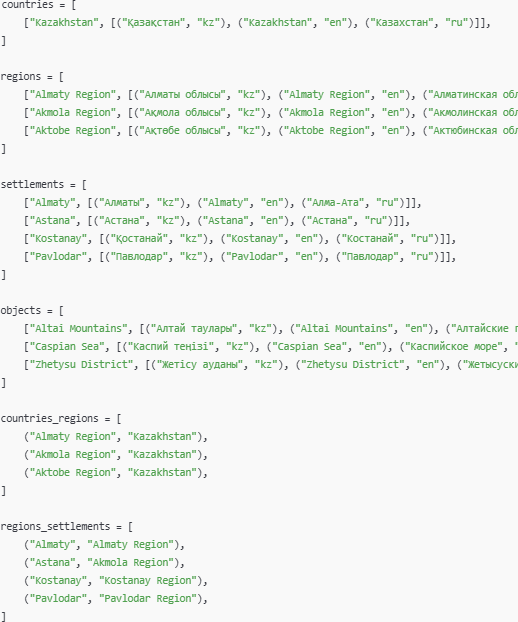
\includegraphics[width=0.6\textwidth]{media/ict2/image153}
	\caption*{Рис.5 - фрагмент промежуточных данных из текста страницы}
\end{figure}

\begin{multicols}{2}
В ответе модели словари и списки соответствуют заданной структуре. Это
имеет несколько важных преимуществ:

- ввод данных непосредственно в обработчик без дополнительных процедур
преобразования;

- OWLready2 очень совместим с другими инструментами для создания
онтологий;

- Масштабируемость и универсальность позволяют использовать полученные
данные в различных областях.

Благодаря этому формату данные из ChatGPT-3.5 могут быть автоматически
импортированы в онтологическую модель.

Иерархические связи и семантическая корректность сохраняются.

Это делает процесс создания онтологии более независимым и эффективным.

Для автоматизации процессов структурирования знаний и демонстрации
практического применения предложенной технологии разработана
онтологическая модель. Эта идея описывает географию страны и ее
административное деление.

Создается иерархическая структура классов и свойств. Модель обеспечивает
формальное машиночитаемое представление важных географических объектов и
их взаимосвязей.
\end{multicols}

\begin{figure}[H]
	\centering
	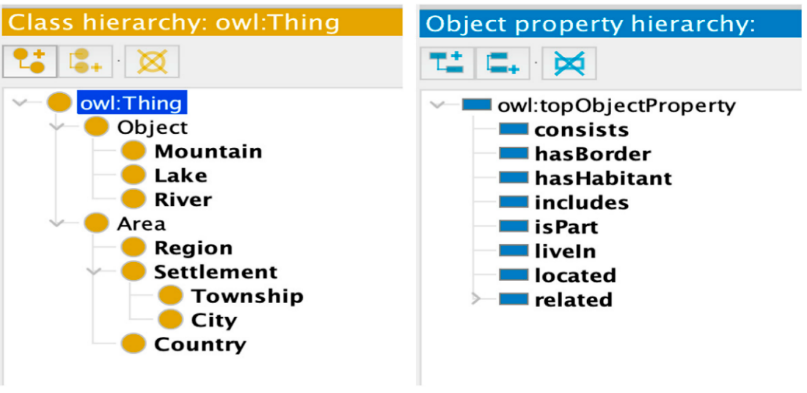
\includegraphics[width=0.6\textwidth]{media/ict2/image154}
	\caption*{Рис.6 - Иерархия классов и свойств разработанной модели {[}12{]}}
\end{figure}

\begin{figure}[H]
	\centering
	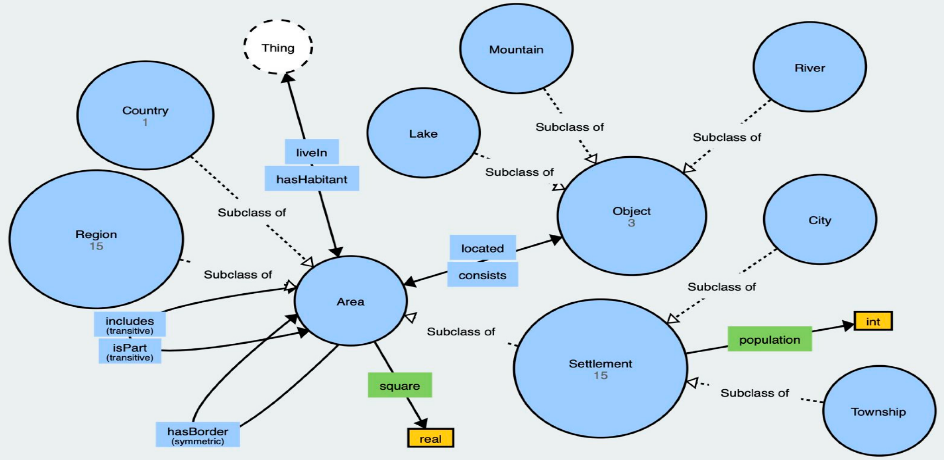
\includegraphics[width=0.8\textwidth]{media/ict2/image155}
	\caption*{Рис.7 - Граф семантической сети геоинформационной системы {[}12{]}}
\end{figure}

\begin{multicols}{2}
Структура онтологической модели показана на рисунке 6. Семантические
характеристики административных единиц представлены их основными
классами, объектными свойствами, свойствами данных. Плагин protégévowl
использовался для создания онтологического графика для визуализации
семантических отношений между объектами. Эта визуализация показана на
рисунке 7. Онтологическая модель была автоматически обновлена
соответствующей информацией путем объединения данных ChatGPT - 3.5.
Кроме того, он расширил сферу своей темы. Таким образом, применение
предложенного метода подтверждает целесообразность динамического
обновления и автоматического синтеза онтологий с использованием данных
из онлайн-источников. В результате система становится семантически
богатой, масштабируемой и адаптивной.

На рисунке 8 представлен код, иллюстрирующий, каким образом в
онтологическую базу вносятся новые элементы. В основе алгоритма ---
создание экземпляров классов с заданием необходимых характеристик. Для
поддержки использования в разных языковых средах каждому элементу
назначаются метки сразу на трёх языках, что позволяет применять модель в
интернациональных условиях.

Такой подход позволяет системе пополнять онтологию автоматически, по
мере появления новых сведений. Это делает систему гибкой и удобной для
адаптации под различные сценарии. Использование данных из
онлайн-источников, имеющих чёткую структуру, помогает более точно
выполнять логические операции и семантический поиск. После запуска
соответствующего скрипта все сущности и их параметры добавляются в
онтологическую модель без участия пользователя.
\end{multicols}

\begin{figure}[H]
	\centering
	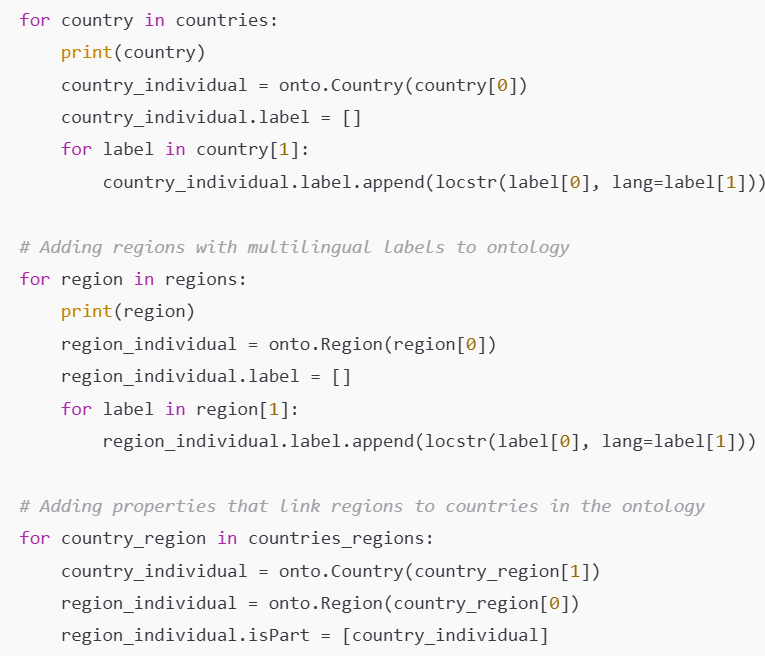
\includegraphics[width=0.6\textwidth]{media/ict2/image156}
	\caption*{Рис.8 - Фрагмент программного кода для создания объектов в онтологии}
\end{figure}

\begin{multicols}{2}
Таким образом, обеспечивается систематическое представление знаний в
соответствии с ранее определенной иерархией классов и характеристик
объектов. Результат, который показывает свойства объектов, структуру
классов и их взаимосвязь, показан на рисунке 9 при обращении к
онтологии, созданной в редакторе protégé.

Как показывает успешный и безошибочный запуск логического механизма
(reasoner), полная логическая совместимость созданной онтологии является
одной из ее основных характеристик. Благодаря такой реализации
онтологическая модель может автоматически обновляться, что значительно
повышает семантическую полноту и точность. Онтология становится
динамичной и может адаптироваться к изменяющимся условиям в предметной
области путем объединения полученных данных. Как таковая, она является
полезным инструментом для приложений семантического поиска и систем
управления знаниями.
\end{multicols}


\begin{figure}[H]
	\centering
	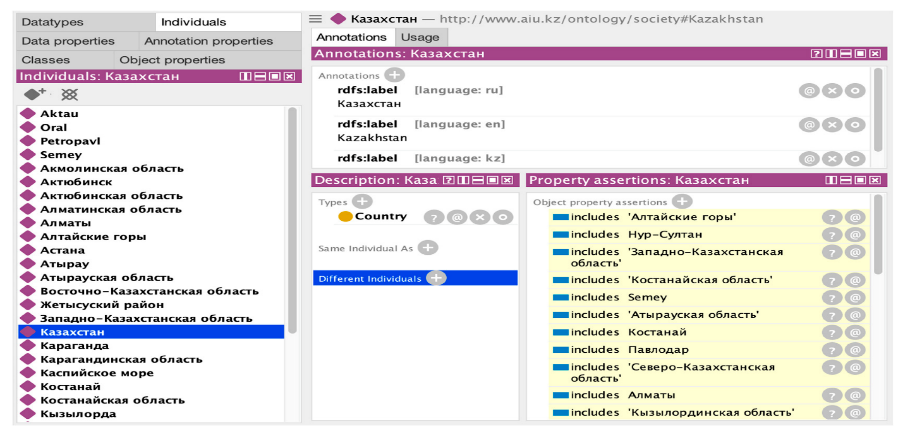
\includegraphics[width=0.8\textwidth]{media/ict2/image157}
	\caption*{Рис.9 - Созданная онтология в редакторе Protégé с инициализированной логикой {[}12{]}}
\end{figure}

\begin{multicols}{2}
{\bfseries Результаты и обсуждение.} Эксперименты проводились для оценки
качества, полноты и продолжительности задачи извлечения данных из
содержимого веб-страницы с использованием ChatGPT 3.5. Целью этих тестов
было проанализировать, насколько хорошо модель автоматически
структурировала информацию и представляла ее в машиночитаемой форме. В
ходе опроса были собраны ключевые параметры извлеченных данных, включая
количество извлеченных объектов, точность, отзыв, F1 и время выполнения
запроса. Результаты представлены в таблице 1. Таблица 1: Результаты
поиска на основе чата 3.5-это данные веб-страниц. Модель поддерживает
приемлемый коэффициент отзыва 0,87 с неизменно высокой степенью точности
в среднем 0,91, согласно результатам анализа.
\end{multicols}

\tcap{Таблица 1 - Результаты экспериментов по извлечению данных с веб-страницы с использованием ChatGPT 3.5}
\begin{longtblr}[
  label = none,
  entry = none,
]{
  width = \linewidth,
  colspec = {Q[180]Q[263]Q[154]Q[131]Q[79]Q[185]},
  cells = {c},
  hlines,
  vlines,
}
Эксперименты & Количество
			извлечённых сущностей & Точность
			(Precision) & Полнота
			(Recall) & F1-score & Время
			выполнения (сек)\\
1 & 120 & 0.89 & 0.85 & 0.87 & 12.4\\
2 & 132 & 0.91 & 0.87 & 0.89 & 11.8\\
3 & 127 & 0.90 & 0.86 & 0.88 & 12.1\\
4 & 135 & 0.92 & 0.88 & 0.90 & 11.5\\
5 & 130 & 0.91 & 0.87 & 0.89 & 11.9
\end{longtblr}

\begin{multicols}{2}
Во время тестирования было замечено, что показатели F1 колебались между
87\% и 90\%. Это связано с тем, что система довольно точно извлекает
данные, при этом средняя полнота остаётся приемлемой. В среднем запрос
обрабатывался за 12 секунд --- благодаря налаженной передаче данных и
стабильной работе API. Автоматизация позволила не только повысить
качество извлекаемой информации, но и ускорила обработку больших
текстов. Модель хорошо себя проявила при работе с различными темами, что
делает её полезной при уточнении и расширении структур знаний.

Таким образом, можно сказать, что ChatGPT 3.5 подходит для задач,
связанных с выделением ключевой информации, а также с созданием
онтологий и упрощением анализа текстовых данных.

{\bfseries Выводы}. Мы проверили, как наш метод справляется с задачей
извлечения информации из обычных текстов. В результате стало ясно, что
он помогает находить важные части текста и включать их в онтологическую
схему. Применение языковых моделей улучшило точность обработки. Пример с
казахским текстом по теме старения показал, что метод работает в разных
тематиках. Мы также заметили, что система подходит для разных форматов
текстов. В будущем мы хотим сделать её более гибкой и точной. Всё это
подтверждает, что предложенный подход полезен для создания систем,
которые умеют переводить обычные тексты в структурированную форму.

\emph{{\bfseries Финансирование}. Данное исследование было проведено
Комитетом науки Министерства науки и высшего образования Республики
Казахстан (грантNo AP19577922) -- «Технология создания интеллектуальной
вопросно-ответной системы на казахском языке».}
\end{multicols}

\begin{center}
{\bfseries Литература}
\end{center}

\begin{references}
1. Ranjan R.,Vathsala H., Koolagudi S.G. Profile generation from web
sources: An information extraction system //
\href{https://link.springer.com/journal/13278}{Social Network Analysis
and Mining}.-2022.-Vol.12(2). DOI 10.1007/s13278-021-00827-y.

2. Jayasankar U., Thirumal V., Ponnurangam D. A survey on data
compression techniques: From the perspective of data quality, coding
schemes, data type and application // Journal of King Saud
University-Computer and Information Science.-2021.-Vol.33(2).-
P.119--140. DOI 10.1016/j.jksuci.2018.05.006.

3. Dey R., Balabantaray R. C., Mohanty S. Sliding window based off-line
handwritten text recognition using edit distance //Multimedia Tools and
Applications. --

2022. -- Vol.81. -- P.22761-22788. DOI
\href{https://link.springer.com/article/10.1007/s11042-021-10988-9}{10.1007/s11042-021-10988-9}.

4. Rupapara V. et al. Relevant data node extraction: A web data
extraction method for non contagious data //2020 5th international
conference on communication and electronics systems (ICCES). - IEEE. -
2020. - P.500-505.
DOI~\href{https://doi.org/10.1109/ICCES48766.2020.9137897}{10.1109/ICCES48766.2020.9137897}.

5. Xu T. et al. Chinese News Data Extraction System Based on Readability
Algorithm //
\href{https://www.researchgate.net/journal/Communications-in-Computer-and-Information-Science-1865-0929?_tp=eyJjb250ZXh0Ijp7ImZpcnN0UGFnZSI6InB1YmxpY2F0aW9uIiwicGFnZSI6InB1YmxpY2F0aW9uIn19}{Communications
in Computer and Information Science}. - 2020. - P.153-164. DOI
\href{http://dx.doi.org/10.1007/978-981-15-8083-3_14}{10.1007/978-981-15-8083-3\_14}

6. Ibrahim S., Fathalla S., Yazdi H., Lehmann J., \& Jabeen H. From
monolingual to multilingual ontologies: The role of cross-lingual
ontology enrichment. // Semantic Systems. The Power of AI and Knowledge
Graphs: 15th International Conference, SEMANTiCS 2019. Lecture Notes in
Computer Science. - 2019. -Vol.11702. Springer. - P.215-230. DOI
10.1007/978-3-030-33220-4\_16.

7. Sanagavarapu L. M., Iyer V., Reddy R. A deep learning approach for
ontology enrichment from \\unstructured text //arXiv preprint
arXiv:2112.08554. - 2021. DOI
\href{http://dx.doi.org/10.48550/arXiv.2112.08554}{10.48550/arXiv.2112.08554}

8. Tissaoui A., Sassi S., Chbeir R. Probabilistic topic models for
enriching ontology from texts //SN Computer Science. -2020. - Vol.1
(336). DOI
\href{https://link.springer.com/article/10.1007/s42979-020-00349-y}{10.1007/s42979-020-00349-y}.

9. Kokla M., Papadias V., Tomai E. Enrichment and population of a
geospatial ontology for semantic information extraction //The
International Archives of the Photogrammetry, Remote Sensing and Spatial
Information Sciences.-2018.-Vol.42. -P.309-314. DOI
\href{http://dx.doi.org/10.5194/isprs-archives-XLII-4-309-2018}{10.5194/isprs-archives-XLII-4-309-2018}

10. Sebubi O., Zlotnikova I., Hlomani H. Ontology-driven semantic
enrichment framework for open data value creation //Data Science
Journal. -2023. -Vol.22. - P.40. DOI
\href{http://dx.doi.org/10.5334/dsj-2023-040}{10.5334/dsj-2023-040}.

11. Hertling S., Paulheim H. Olala: Ontology matching with large language
models //Proceedings of the 12th Knowledge Capture Conference,
2023. -2023.- P.131-139. DOI
\href{http://dx.doi.org/10.1145/3587259.3627571}{10.1145/3587259.3627571}.

12. Mukanova, A., Milosz, M., Dauletkaliyeva, A., Nazyrova, A.,
Yelibayeva, G., Kuzin, D., \& Kussepova, L. LLM-powered natural language
text processing for ontology enrichment. -- 2024. -14(13): 5860. DOI
\href{http://dx.doi.org/10.3390/app14135860}{10.3390/app14135860}.
\end{references}

\begin{authorinfo}
\emph{{\bfseries Сведения об авторах}}

Даулеткалиева А.-докторант Международного университета Астаны, Астана,
Казахстан, e-mail:\\ assem.dauletkaliyeva1@gmail.com;

Муканова А. - PhD, доцент Международного университета Астаны,Астана,
Казахстан, e-mail: asiserikovna@gmail.com;

Назырова А. -- PhD, Евразийский национальный университет им. Л. Н.
Гумилева, старший преподаватель кафедры «технологии искусственного
интеллекта», Астана, Казахстан, e-mail: ayzhan.nazyrova@gmail.com;

Ергеш Б. - PhD, заместитель директора департамента цифрового развития
Евразийского национального университета им. Л. Н. Гумилева, Астана,
Казахстан, e-mail: b.yergesh@gmail.com;

Жеткенбай Л. - PhD, Евразийский национальный университет им. Л. Н.
Гумилева, старший преподаватель кафедры «технологии искусственного
интеллекта», Астана, Казахстан, e-mail: jetlen7@gmail.com;

Бурибаева А. - PhD, доцент Международного университета Астаны, Астана,
Казахстан, e-mail: buribayeva@mail.ru.

\emph{{\bfseries Information about the authors}}

Dauletkaliyeva A.- doctoral student at Astana International
University,Astana, Kazakhstan e-mail:\\
assem.dauletkaliyeva1@gmail.com;

Mukanova A. - PhD, аssoc. professor of the Astana International
University, Astana, Kazakhstan, e-mail: \\asiserikovna@gmail.com;

Nazyrova A. -- PhD, L. N. Gumilyov Eurasian National University, senior
lecturer of the Department of artificial intelligence technologies,
Astana, Kazakhstan, e-mail: ayzhan.nazyrova@gmail.com;

Yergesh B. - PhD, L. N. Gumilyov Eurasian National University, deputy
director of the Department of digital development, Astana, Kazakhstan,
e-mail: b.yergesh@gmail.com;

Zhetkenbai L. - PhD, L.N. Gumilyov Eurasian National University, senior
lecturer of the Department of artificial intelligence technologies,
Astana, Kazakhstan, e-mail: jetlen7@gmail.com;

Buribayeva A. - PhD, Associate Professor at Astana International
University,Astana, Kazakhstan, e-mail: buribayeva@mail.ru.
\end{authorinfo}
